\documentclass[a4paper, 11pt, oneside]{scrartcl}
\usepackage{lpp}
\usepackage{graphicx}
\usepackage{tikz}
\usetikzlibrary{shapes.geometric, arrows}

\begin{document}

\mtitle{Unstructured FEM}

\mauthor{Mohsin Ali Chaudry, Raghavan Lakshmanan, Abhishek Y. Deshmukh}{A. Emre Ongut}

\maff{SiSc Laboratory}{a.deshmukh@grs-sim.de}{ongut@cats.rwth-aachen.de}

\mabstract{This engineering project of SiSc Lab involves the development of a parallel finite element
solver using unstructured grids. The developed and optimized code is validated using
analytical solutions and then it will be parallelized and used to solve a time-dependent engineering heat
transfer problem. 
}

\section{Introduction}

\nocite{midsummer}
Finite element method(FEM) is numerical procedure that is used to obtain solutions of variety of engineering problems like stress analysis, fluid flow, heat transfer, etc.In this project, we are particularly using FEM to solve heat transfer problem for unstructured mesh for steady and unsteady 2D case.

Finite element implementation can generally be divided into following steps:

\subsection{Preprocessing}
\begin{itemize}
\item Discretization of domain into finite elements which comprises of nodes and elements
\item We then have to specify a shape function to represent physical behaviour of element
\item Construct local stiffness matrix and then ultimately global stiffness matrix
\item Then we have to apply boundary condition, initial conditions and loading (forcing function)
\end{itemize}

\subsection{Solution Phase}
\begin{itemize}
\item  Solving linear system of algebraic equations to obtain nodal results.
\end{itemize}


\subsection{PostProcessing Phase}
\begin{itemize}
\item  Postprocess the results. For instance, visualizing temeprature distribution using Paraview, generating plots by extracting relevant information.
\end{itemize}

\section{Finite Element Formulation: Unsteady State}
We are going to model transient heat diffusion equation. This model can also be used to predict the steady state if we let it run for sufficiently large time.

\subsection{1D Heat Diffusion Equation}
One dimensional unsteady heat diffusion equation with some forcing function can be written as

$$\frac{\partial T}{\partial t}-k \frac{\partial^2T}{\partial x^2} =f , \text{in }  \Omega \in \Re $$ 
where k is diffusion coefficient.

In order to solve this unsteady problem, we apply semi-discretization, in which forward euler method is used to discretize through time. In addition, we need two boundary conditions and one initial condition.

Here, temeprature evolves in time and space. We apply weighted residual method.

 $$\int_\Omega (w \frac{\partial T}{\partial t}  +k w\frac{\partial^2 T}{\partial x^2})dx= \int_\Omega wfdx $$
 
where w is a weigthing function or test function.
Integrating by parts and rearranging the terms,
 $$\int_\Omega (w \frac{\partial T}{\partial t}  +k\frac{\partial w}{\partial x}\frac{\partial T}{\partial x})dx= \int_\Omega wfdx+\int_ \Gamma (wk \frac{\partial T}{\partial x}n_x)d \Gamma $$
\begin{figure}[ht!]
\centering
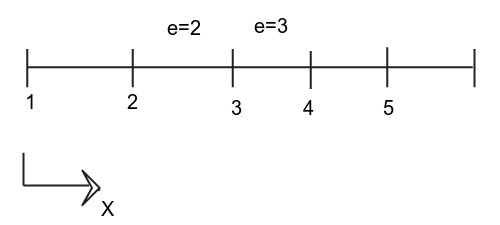
\includegraphics[width=70mm]{element.jpeg}
\caption{Stencil of element}

\end{figure}

 \textbf{Intial and Boundary Conditions:}
 
 The initial distribution of temperature over the domain $\Omega$ can be provided. 
 $$T(x,0) = T_{initial}(x)$$
 
 Boundary conditions can be of three types:

 Dirichlet: $$T(0,t) = T_L$$ $$T(L,t) = T_R$$ where temperature at boundary nodes is known.


 Neumann: $$k\frac{\partial T}{\partial x} n_x = q_0$$ where heat flux going in or out of the boundary is known.


 Robin(Mixed): $$h(T - T_{\infty}) = -k\frac{\partial T}{\partial x}$$ where the temperature of the free stream fluid ($T_{\infty}$) and correspoding heat transfer coefficient(h) is known.
 
\begin{itemize}
\item Approximate solution: We approximate the temperature as a piecewise linear combination of shape functions $S_j(x)$. These shape functions remain constant over time, so the coefficients $T_j(t)$ are time dependent.
 \end{itemize}
 $${ T }_{ app }(x,t)=\sum _{ j=1 }^{ nn }{ { T }_{ j }(t){ S }_{ j }(x) } $$
 
\begin{figure}
\centering
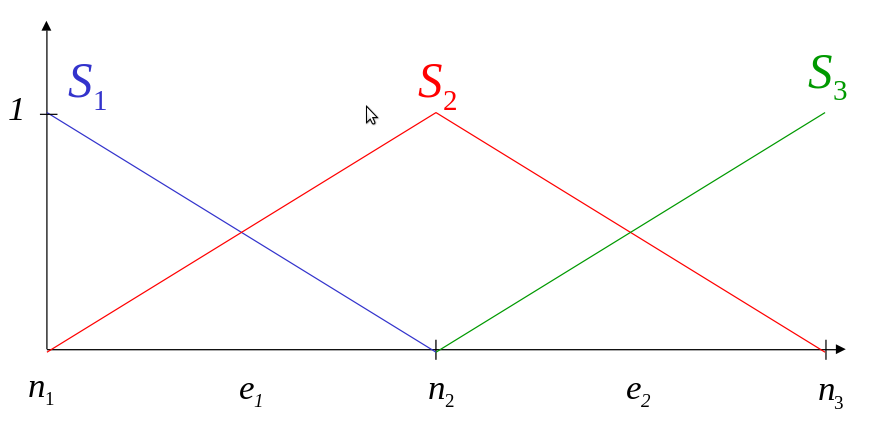
\includegraphics[scale=0.3]{./hat_fun.png}
\caption{Shape functions}
\end{figure}
$$ \int_\Omega [w\sum_{j=1}^{nn} \frac{dT_j}{dt}S_j +k \frac{dw}{dx}(\sum_{j=1}^{nn}T_j\frac{dS_j}{dx})]dx=\int_\Omega wfdx+\int_\Gamma w(k\frac{\partial T}{\partial x})d\Gamma$$

\begin{itemize}
\item Galerkin Finite Element Method: Here weight functions are taken as $$w=S_i(x)$$
\end{itemize}
$$\int_\Omega [S_i\sum_{j=1}^{nn} \frac{dT_j}{dt}S_j +k \frac{dS_i}{dx}(\sum_{j=1}^{nn}T_j\frac{dS_j}{dx})]dx=\int_\Omega S_ifdx+\int_\Gamma S_i(k\frac{\partial T}{\partial x})d\Gamma$$

By taking summation outside of integral for i=1,2,...,nn
$$\underbrace{\sum_{j=1}^{nn} \int_\Omega (S_i S_j)dx\frac{dT_j}{dt}}_{[M][\dot T]} +\underbrace{\sum_{j=1}^{nn}[\int_\Omega(k \frac{dS_i}{dx}\frac{dS_j}{dx})dx]T_j}_{[K][T]}=\underbrace{\int_\Omega S_ifdx}_{[F]} + \underbrace{\int_\Gamma S_i(k\frac{\partial T}{\partial x})d\Gamma}_{[B]}$$

In matrix form we can write it as:
$$[M][\dot{T}]+[K][T]=[F]+[B]$$

Forward Euler expicit differencing in time:

$$ \frac{dT}{dt } \mid_s = \frac{T^{s+1}-T^s}{ \Delta t} +O( \Delta t)$$

$$[M]^s  \frac{[T]^{s+1}-[T]^s}{ \Delta t} +[K]^s[T]^s=[F]^s+[B]^s$$

$$[M] [T]^{s+1}=[M][T]^s+{ \Delta t} ([F]+[B]-[K][T]^s)$$


Backward Euler, Implicit differencing in time:

$$ \frac{dT}{dt } \mid_{s+1} = \frac{T^{s+1}-T^s}{ \Delta t} +O( \Delta t)$$

$$ [M]^{s+1}\frac{T^{s+1}-T^s}{ \Delta t} +[K]^{s+1}[T]^{s+1}=[F]^{s+1}+[B]^{s+1}$$

$$[M] [T]^{s+1}=[M][T]^s+{ \Delta t} ([F]+[B]-[K][T]^{s+1})$$

Stencil in time can be viewed as :

\begin{figure}[ht!]
\centering
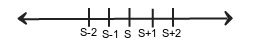
\includegraphics[width=70mm]{stencil.jpeg}
\caption{Time level stencil}

\end{figure}

We use forward euler differencing scheme here.


$$\left[ M \right] { \left[ T \right]  }^{ s+1 }=\left[ M \right] { \left[ T \right]  }^{ s }+\Delta t(\left[ F \right] +\left[ B \right] -\left[ K \right] { \left[ T \right]  }^{ s })$$

$$\begin{pmatrix} * & * & \quad  & \quad  & \quad  \\ \quad * & * & * & \quad  & \quad \quad  \\ \quad  & * & M & * & \quad  \\ \quad  & \quad  & * & * & * \\ \quad  & \quad  & \quad  & * & * \end{pmatrix}\\ \quad {\begin{bmatrix} T_{ 1 } \\ . \\ . \\ . \\  T_{ nn } \end{bmatrix} }^{ s+1 }=\begin{pmatrix} * & * & \quad  & \quad  & \quad  \\ \quad * & * & * & \quad  & \quad \quad  \\ \quad  & * & M & * & \quad  \\ \quad  & \quad  & * & * & * \\ \quad  & \quad  & \quad  & * & * \end{pmatrix}\\ \quad {\begin{bmatrix} T_{ 1 } \\ . \\ . \\ . \\  T_{ nn } \end{bmatrix} }^{ s } + .. $$


$$.. \Delta t({\begin{bmatrix} F_{ 1 } \\ . \\ . \\ . \\ . \\  F_{ nn } \end{bmatrix} } + {\begin{bmatrix} T_{ L } \\ . \\ . \\ . \\ . \\  T_{ R } \end{bmatrix} }- \begin{pmatrix} 1 & 0 & 0  & \quad  & \quad  \\ \quad * & * & * & \quad  & \quad \quad  \\ \quad  & * & K & * & \quad  \\ \quad  & \quad  & * & * & * \\ \quad  & \quad  & \quad  & 0 & 1 \end{pmatrix}\\ \quad {\begin{bmatrix} T_{ L } \\ . \\ . \\ . \\ . \\  T_{ R } \end{bmatrix} }^{ s }) $$

This generally results in a linear system with sparse mass matrix M on the left hand side and a right hand side. On solving this system, we can predict the temperature values at nodes at the time level $s+1$
$$[M][T]^{s+1} = [RHS]^{s}$$
The inversion of Mass matrix can be avoided if we do a physical approximation. This procedure is called lumping of mass matrix.

Lumped mass matrix

Consistent element  mass matrix $$[M_{cij}]$$
Lumped element mass matrix $$[M_{Lij}]$$	

We scale diagonal elements of consistent  mass matrix such that the total mass 	remains same.

$${ M }_{ Lii }={ M }_{ cii }\frac { \sum _{ i=1 }^{ n }{ \sum _{ j=1 }^{ n }{ { M }_{ cij } }  }  }{ \sum _{ j=1 }^{ n }{ { M }_{ cjj } }  }$$	  

This is correct only for linear elements.

\subsection{2D heat Diffusion Equation}
Two dimensional unsteady heat diffusion equation with some forcing function can be written as

$$\frac{\partial T}{\partial t}-k \nabla^2T =f , \text{in }  \Omega \in \Re^2 $$ 
where k is diffusion coefficient.

Similar to 1D formulation, we apply weighted residual method.

 $$\int_\Omega (w \frac{\partial T}{\partial t}  +k w\nabla^2T)d\Omega= \int_\Omega wfd\Omega $$
 
where w is a weigthing function or test function.
Integrating by parts and applying Gauss divergence theorem,
 $$\int_\Omega (w \frac{\partial T}{\partial t}  +k\nabla w .\nabla T)d\Omega = \int_\Omega wfd\Omega + \int_ \Gamma w\underbrace{(k \hat{n}.\nabla T)}_{k(n_x\frac{\partial T}{\partial x} + n_y\frac{\partial T}{\partial y})}d\Gamma $$

Again, we approximate the temperature as a piecewise linear combination of shape functions $S_j(x,y)$. These shape functions remain constant over time, so the coefficients $T_j(t)$ are time dependent.

 $${ T }(x,y,t)=\sum _{ j=1 }^{ nn }{ { T }_{ j }(t){ S }_{ j }(x,y) } $$

Galerkin Finite Element Method: $$w=S_i(x)$$

$$\sum_{j=1}^{nn} \int_\Omega (S_i S_j)d\Omega \frac{\partial T_j}{\partial t} - \sum_{j=1}^{nn}[\int_\Omega k(\frac{\partial S_i}{\partial x}\frac{\partial S_j}{\partial x} + \frac{\partial S_i}{\partial y}\frac{\partial S_j}{\partial y})d\Omega] T_j = \int_\Omega S_i	f d\Omega  +  \int_\Gamma S_i (k \hat{n}.\nabla T) d\Gamma$$
$$K_{ij} = \int_\Omega k(\frac{\partial S_i}{\partial x}\frac{\partial S_j}{\partial x} + \frac{\partial S_i}{\partial y}\frac{\partial S_j}{\partial y})d\Omega$$
$i,j = 1,2,...,nn $

\textbf{2D Master Element:}

In 2D, two types of elements can be used, namely, triangular or quads depending on the mesh being used to solve upon. We have implemented for tri-elements.
\begin{figure}[ht!]
\centering
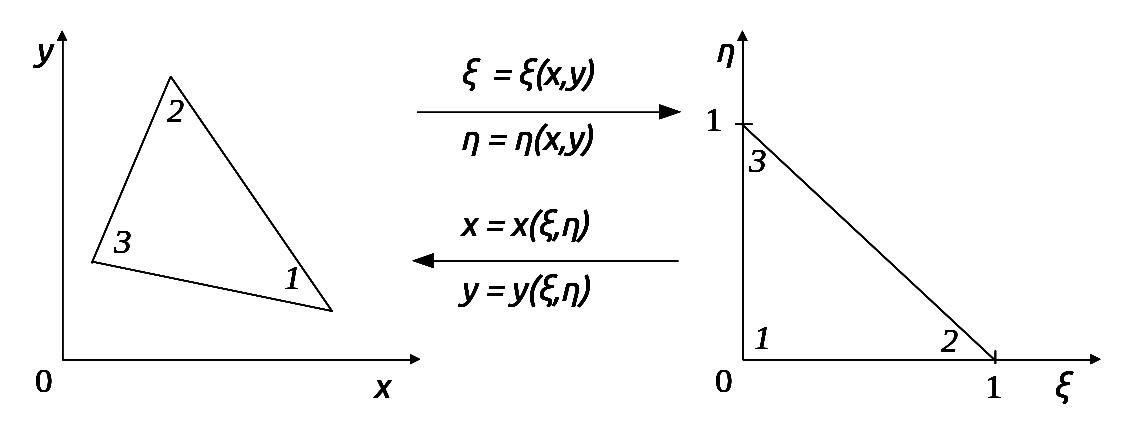
\includegraphics[width=140mm]{master_elem.png}
\caption{Co-ordinate transformation}
\end{figure}

$$S_1(\xi,\eta) = 1 - \xi - \eta$$ $$S_2(\xi,\eta) = \xi$$ $$S_3(\xi,\eta) = \eta$$

$$\frac{\partial S_1}{\partial \xi} = -1  ,    \frac{\partial S_2}{\partial \xi} = 1 ,   \frac{\partial S_3}{\partial \xi} = 0,   \frac{\partial S_1}{\partial \eta} = -1,    \frac{\partial S_2}{\partial \eta} = 0,     \frac{\partial S_3}{\partial \eta} = 1$$

$$\frac{\partial S_i}{\partial \xi} = \frac{\partial S_i}{\partial x}\frac{\partial x}{\partial \xi} + \frac{\partial S_i}{\partial y}\frac{\partial y}{\partial \xi}, \frac{\partial S_i}{\partial \eta} = \frac{\partial S_i}{\partial x}\frac{\partial x}{\partial \eta} + \frac{\partial S_i}{\partial y}\frac{\partial y}{\partial \eta}$$

$$\begin{bmatrix}
\frac{\partial S_i}{\partial \xi} \\ \\ \frac{\partial S_i}{\partial \eta}
\end{bmatrix} = \underbrace{\begin{bmatrix}
\frac{\partial x}{\partial \xi} \quad \frac{\partial y}{\partial \xi}\\ \\ \frac{\partial x}{\partial \eta} \quad \frac{\partial y}{\partial \eta} 
\end{bmatrix}}_{Jacobian} \begin{bmatrix}
\frac{\partial S_i}{\partial x} \\ \\ \frac{\partial S_i}{\partial y}
\end{bmatrix}$$

\textbf{Isoparametric formulation:}
$$x(\xi,\eta) = \sum_{j=1}^{nen} x_j^e S_j(\xi,\eta) \text{ , }
 y(\xi,\eta) = \sum_{j=1}^{nen} y_j^e S_j(\xi,\eta)$$
 Using above formulation, we can write Jacobian as:
 $$\begin{bmatrix}J\end{bmatrix} = \begin{bmatrix}
\frac{\partial S_1}{\partial \xi} \quad \frac{\partial S_2}{\partial \xi}\quad \frac{\partial S_3}{\partial \xi}\\ \\ \frac{\partial S_1}{\partial \eta} \quad \frac{\partial S_2}{\partial \eta}\quad \frac{\partial S_3}{\partial \eta} 
\end{bmatrix} \begin{bmatrix}
x_1^e \quad y_1^e\\ \\ x_2^e \quad y_2^e \\ \\ x_3^e \quad y_3^e\end{bmatrix} = \begin{bmatrix}
\frac{\partial x}{\partial \xi} \quad \frac{\partial y}{\partial \xi}\\ \\ \frac{\partial x}{\partial \eta} \quad \frac{\partial y}{\partial \eta} 
\end{bmatrix}$$
But we need $[J]^{-1}$ which is the inverse mapping. 
$$\begin{bmatrix}
\frac{\partial S_i}{\partial x} \\ \\ \frac{\partial S_i}{\partial y}
\end{bmatrix} = \underbrace{\begin{bmatrix}
\frac{\partial \xi}{\partial x} \quad \frac{\partial \eta}{\partial x}\\ \\ \frac{\partial \xi}{\partial y} \quad \frac{\partial \eta}{\partial y} 
\end{bmatrix}}_{[J]^{-1}}\underbrace{\begin{bmatrix}
\frac{\partial S_i}{\partial \xi} \\ \\ \frac{\partial S_i}{\partial \eta}
\end{bmatrix}}_{known} $$
\textbf{Calculation of element level stiffness matix:}
$$K_{ij}^e = \int_{\Omega_e} k(\frac{\partial S_i}{\partial x}\frac{\partial S_j}{\partial x} + \frac{\partial S_i}{\partial y}\frac{\partial S_j}{\partial y})dx dy \text{     i,j = 1,2,...,nn}$$
Integral transformation to master element:
$$K_{ij}^e = \int_{0}^1 \int_0^{1-\xi} \underbrace{k[(\frac{\partial S_i}{\partial \xi}\frac{\partial \xi}{\partial x} + \frac{\partial S_i}{\partial \eta}\frac{\partial \eta}{\partial x})(\frac{\partial S_j}{\partial \xi}\frac{\partial \xi}{\partial x} + \frac{\partial S_j}{\partial \eta}\frac{\partial \eta}{\partial x}) + (\frac{\partial S_i}{\partial \xi}\frac{\partial \xi}{\partial y} + \frac{\partial S_i}{\partial \eta}\frac{\partial \eta}{\partial y})(\frac{\partial S_j}{\partial \xi}\frac{\partial \xi}{\partial y} + \frac{\partial S_j}{\partial \eta}\frac{\partial \eta}{\partial y})]|J|}_{Integrand := f_k(\xi,\eta)}d\xi d\eta$$
$i,j = 1,2,...,nn$

The integration is done numerically using Gauss Quadrature rule. We have used 7 point Gauss Quadrature rule.
$$K_{ij}^e \simeq \sum_{i=1}^{nGQP}f_k(\xi_i,\eta_i) w_i$$

These points are shown in figure 5.
\begin{figure}[ht!]
\centering
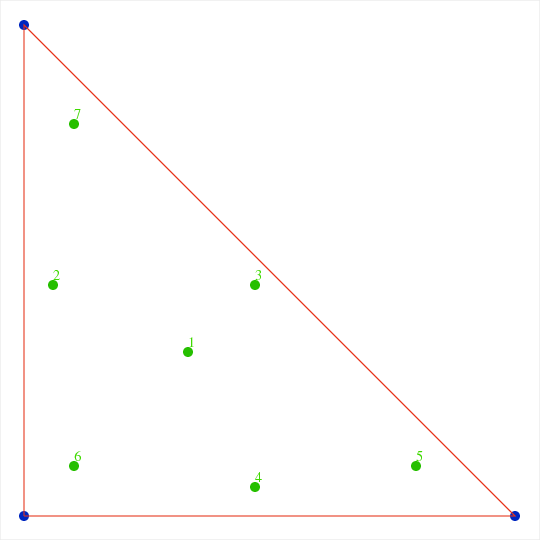
\includegraphics[width=40mm]{GQP7.png}
\caption{7 Gauss Quadrature Points}
\end{figure}
Similarly, element level mass matrix [M] and source term [S] is also calculated by numerical integration.
\\
\\
\textbf{Boundary Integral:}
\\
According to the boundary conditions, we determine the components of boundary integral. For the nodes where the essential boundary conditions($T=T_w$) are given, we don't need to evaluate the boundary integral. We can specify $T_w$ in boundary integral and make necessay changes in [K] matrix. For example, if for some element, node temperatures T1 and T3 are known then [B] and [K] for that element can be written as:
$$[B] = \begin{bmatrix}
T_w \\
B_2 \\
T_w
\end{bmatrix} \text{  and  } [K] = \begin{bmatrix}
1 \quad 0 \quad 0 \\
\ast \quad \ast \quad \ast \\
0 \quad 0 \quad 1
\end{bmatrix} $$  In addition, for the nodes on insulated wall there is no contribution to the boundary integral since the heat flux at these nodes is zero. We need to evaluate the boundary integral in case of Neumann and Robin(Mixed) boundary conditions where explicit heat flux is given. We need to evaluate this integral on the edges of the elements which lie on one of these boundaries. Over the edge the 2D shape functions reduce to 1D shape functions as it can be seen in the figure 6.\\
$S_1$ and $S_2$ can be clearly written as $S_1 = 1- \frac{r}{L}$ , $S_2 = \frac{r}{L}$
\begin{figure}[ht!]
\centering
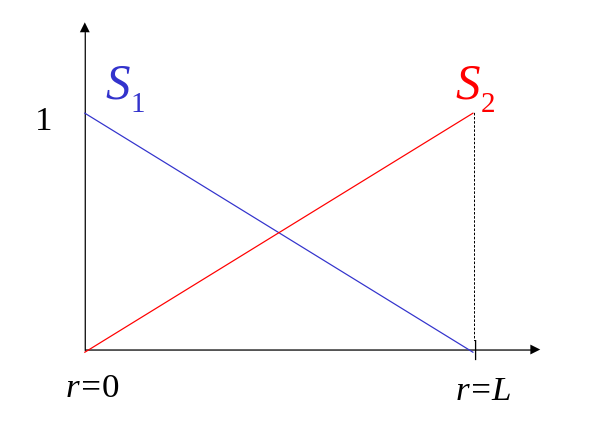
\includegraphics[width=50mm]{edge_shape_fun.png}
\caption{Shape functions over the edge of tri-element}
\end{figure}
\\
For Neumann Boundary conditions (Flux Variable(FV) = $q_{in}$):
\\
$$B_1^e = \int_\Gamma S_1 (FV)d\Gamma = \int_0^L (1-\frac{r}{L}) q_{in}dr = \frac{q_{in} L}{2} $$
$$B_2^e = \int_\Gamma S_2 (FV)d\Gamma = \int_0^L \frac{r}{L} q_{in}dr = \frac{q_{in} L}{2} $$

$$[B] = \begin{bmatrix}
\frac{q_{in}L}{2} \\
\frac{q_{in}L}{2} \\
0
\end{bmatrix}$$ 
For Robin(Mixed type) Boundary conditions:
Flux variable can be expressed as $$-k \hat{n}.\nabla T = h(T - T_{\infty})$$
$FV = a PV + b$ where a = -h and b = $hT_{\infty}$

$$B_1^e = \int_\Gamma S_1 (FV)d\Gamma = \int_0^L (1-\frac{r}{L}) (a PV + b)dr$$
$$B_2^e = \int_\Gamma S_2 (FV)d\Gamma = \int_0^L \frac{r}{L} (a PV + b)dr$$
Primary variable temperature appears inside the integrals. We can express temperature in terms of shape functions $S_1$ and $S_2$ and evaluate the boundary integrals.
$$PV = S_1 T_1 + S_2 T_2$$
$$B_1^e = \int_0^L (1-\frac{r}{L})[a ((1-\frac{r}{L})T_1 + \frac{r}{L}T_2 ) + b]dr = \frac{L}{6}(3b + 2aT_1 + aT_2)$$
$$B_2^e = \int_0^L \frac{r}{L}[a ((1-\frac{r}{L})T_1 + \frac{r}{L}T_2 ) + b]dr = \frac{L}{6}(3b + aT_1 + 2aT_2)$$
and element boundary vector can be written as:
$$[B] = \begin{bmatrix}
\frac{L}{6}(3b + 2aT_1 + aT_2) \\
\frac{L}{6}(3b + aT_1 + 2aT_2) \\
0
\end{bmatrix}$$
As the temperature which is unknown here, appears in the boundary integral, we have to rearrange [B] and [K] and transfer coefficients unknown primary variables to [K]. Modified [B] and corresponding [K] can be written as:
$$[B] = \begin{bmatrix}
\frac{Lb}{2} \\
\frac{Lb}{2} \\
0
\end{bmatrix} \text{  and  } [K] = \begin{bmatrix}
(\ast - \frac{aL}{3}) \quad (\ast - \frac{aL}{6}) \quad \quad \ast \\
(\ast - \frac{aL}{6}) \quad (\ast - \frac{aL}{3}) \quad \quad \ast \\
\ast \quad \quad \quad \quad \ast \quad \quad \quad \quad \ast
\end{bmatrix} $$
Rest of the procedure to evaluated the temperature at new time level from previous time level is similar to one dimenional formulation.

\section{Implementation}
 The solver has been implemented in Object Oriented C++ Code. The detailed documentation has been generated using Doxygen. Overall program flow is shown in figure 7.
% Define the styles for each block
\tikzstyle{startstop} = [rectangle, rounded corners, minimum width=3cm, minimum height=1cm,text centered, draw=black, fill=red!30]
\tikzstyle{io} = [trapezium, trapezium left angle=70, trapezium right angle=110, minimum width=3cm, minimum height=1cm, text centered, draw=black, fill=blue!30]
\tikzstyle{process} = [rectangle, minimum width=3cm, minimum height=1cm, text centered, draw=black, fill=orange!30]
\tikzstyle{decision} = [diamond, minimum width=3cm, minimum height=1cm, text centered, draw=black, fill=green!30]
\tikzstyle{arrow} = [thick,->,>=stealth]

%<TikZ code>
\begin{figure}

\begin{center}
\begin{tikzpicture}[node distance=2cm]

% Nodes
\node (start) [startstop] {Start};
\node (in1) [io, below of=start, minimum width=2cm, minimum height=1cm, text centered, text width=6cm, draw=black, yshift=-0.5cm] {Input: Mesh files, Initial and Boundary conditions, Diffusion Coefficient, Source term, No. of iterations, Time step, Data Writing Frequency};
\node (pro1) [process, below of=in1, yshift=-0.5cm] {Define Mesh Structures};
\node (pro2) [process, below of=pro1, minimum width=5cm, minimum height=1cm, text centered, text width=5cm, draw=black] {Calculate Metrics: Jacobian, Element level Matrices};
\node (pro2z) [process, below of=pro2, minimum width=4cm, minimum height=1cm, text centered, text width=3cm, draw=black] {Apply Boundary Conditions};
%\node (dec1) [decision, below of=pro1, yshift=-0.5cm] {Decision 1};
\node (pro2a) [process, below of=pro2z,  minimum width=3cm, minimum height=1cm, text centered, text width=5cm, draw=black] {Solver: Solve 2D Heat diffusion equation};
%\node (pro2b) [process, right of=pro1, xshift=2cm] {Process 2b};
\node (pro2b) [io, below of=pro2a, minimum width=3cm, minimum height=1cm, text centered, text width=2cm, draw=black] {Write VTK Data};
\node (pro2c) [process, right of=pro2b, xshift=2cm] {time+=dt};
\node (dec1) [decision, below of=pro2b, yshift=-0.5cm] {iter<NIter};
%\node (out1) [io, below of=dec1, yshift=-0.5cm, minimum width=3cm, minimum height=1cm, text centered, text width=3cm, draw=black] {Output in Paraview};
\node (stop) [startstop, below of=dec1, yshift=-0.5cm] {Stop};

% Arrows
\draw [arrow] (start) -- (in1);
\draw [arrow] (in1) -- (pro1);
%\draw [arrow] (pro1) -- (dec1);
%\draw [arrow] (dec1) -- (pro2a);
%\draw [arrow] (dec1) -- (pro2b);
\draw [arrow] (pro1) -- (pro2);
\draw [arrow] (pro2) -- (pro2z);
\draw [arrow] (pro2z) -- (pro2a);
\draw [arrow] (pro2a) -- (pro2b);
\draw [arrow] (pro2b) -- (dec1);
\draw [arrow] (dec1) -- node[anchor=east] {no} (stop);
\draw [arrow] (dec1) -| node[anchor=south] {yes} (pro2c);
\draw [arrow] (pro2c) |- (pro2a);
%\draw [arrow] (out1) -- (stop);

\end{tikzpicture}\\
\end{center}
\caption{Overall Program Flow Chart}
\end{figure}
\section{Verification and Validation}
Verification and validation of the code is done against analytical solution found in \cite{jw}. 

\subsection{Case: 1D}
A simple 1D case is taken as an example.
Initial condition: $T_i = T(x,0) = 1000 K$
\\
Boundary Conditions: $T_L = T(0,t)) = 0$, 
$T_R = T(L,t)) = 0$, $T_{top}$ and $T_{bottom}$ are insulated
\\
Analytical Solution: $$T(x,t) = \sum_{n=1}^{\infty} B_n sin(\frac{n \pi x}{L}) e^{-\frac{n^2 \pi^2 \alpha t}{L^2}} $$ where $\alpha$ is diffusion coefficient and  $$B_n = -T_i \frac{2(-1 + (-1)^n)}{n\pi}$$

\begin{figure}[ht!]
\centering
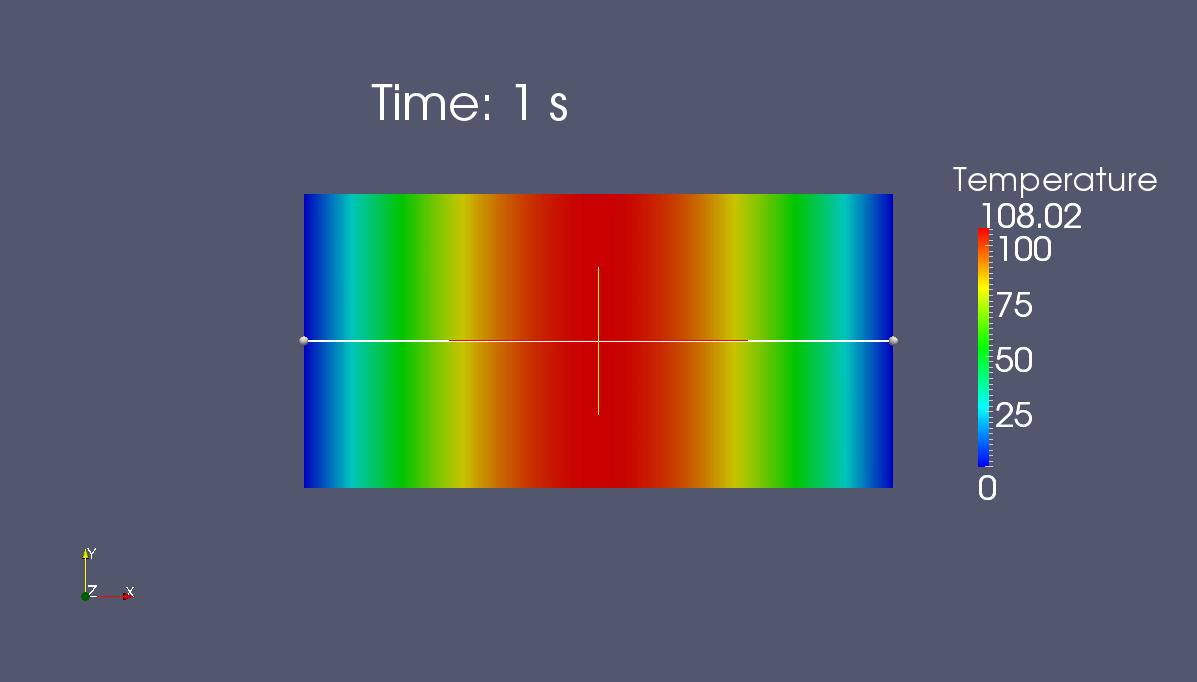
\includegraphics[width=120mm]{./Output/1D_paraview.png}
\caption{1D: Paraview Output}
\end{figure}

\begin{figure}[ht!]
\centering
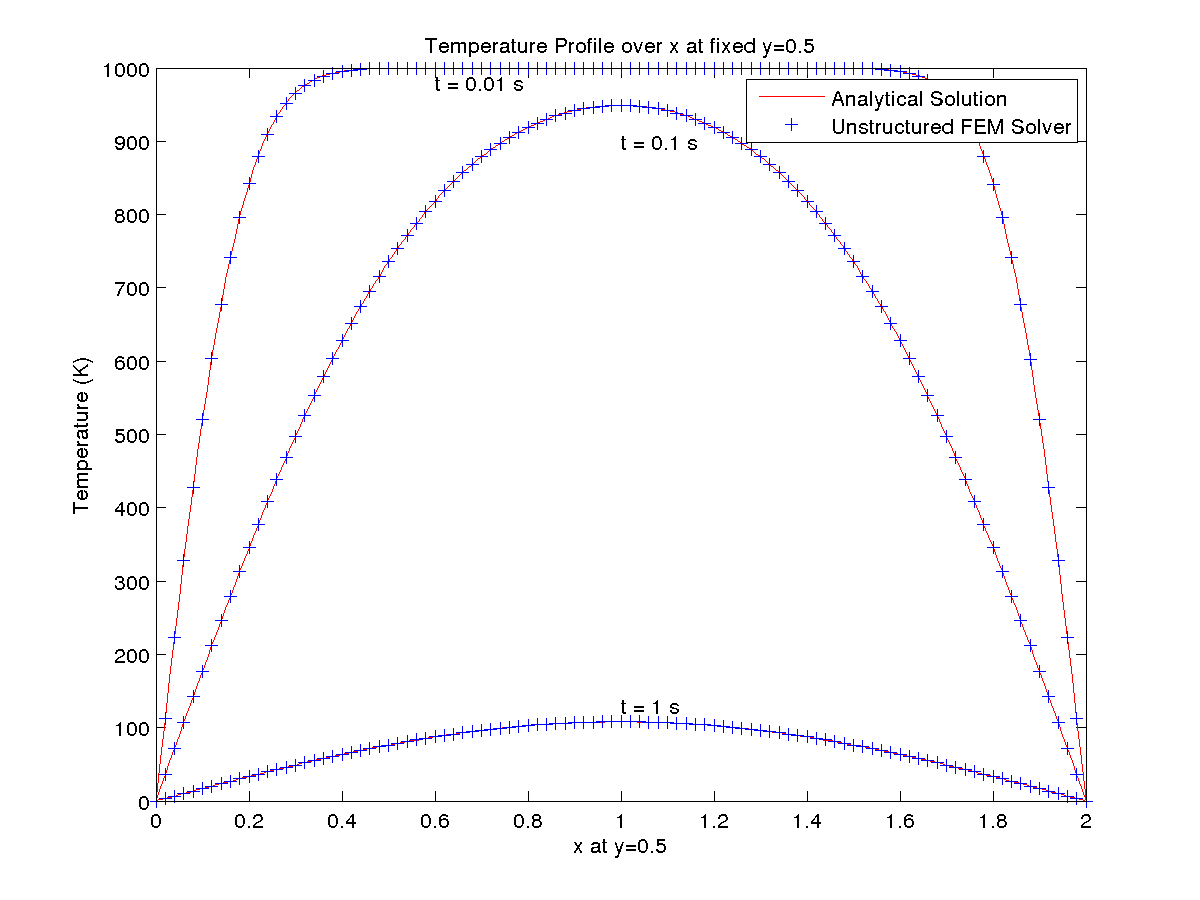
\includegraphics[width=150mm]{./Output/1D.png}
\caption{1D: Comparison with Analytical solution}
\end{figure}
As we can see from figure 9, there is excellent match of the numerical solution with analytical solution at each time level.
\subsection{Case: 2D Quenching of a Billet {\cite{jw}}}
Consider a long billet of rectangular cross section $2a \times 2b$ initially at a uniform temperature $T_i$ which is quenched by exposing it to convective exchange with an environment at $T_{\infty}$ by means of a heat transfer coefficient h. Since the billet is long it is appropriate to neglect conduction along its axis. Because of symmetry it is enough to analyze one quarter of the cross section using a rectangular Cartesian system of coordinates with the origin at the center of the billet. 
\\
Define a shifted temperature, $\theta(x,y,t) = T(x,y,t) - T_{\infty}$
\\
Initial condition: $\theta (x,y,0) = T_i - T_{\infty} = \theta_i$
\\
Boundary Conditions: At $x = 0$, $$\frac{\partial \theta}{\partial x} = 0$$
At $x = a$, $$\frac{\partial \theta}{\partial x} = -\frac{h}{k} \theta (a,y,t)$$
At $y = 0$, $$\frac{\partial \theta}{\partial y} = 0$$
At $y = b$, $$\frac{\partial \theta}{\partial y} = -\frac{h}{k} \theta (x,b,t)$$
\\
In terms of the shifted temperature the analytical solution of the problem is as follows: $$\frac{\theta}{\theta_i} = 4 \sum_{n=1}^{\infty} \sum_{m=1}^{\infty} e^{(-\alpha(\lambda_n^2 + \beta_m^2) t)}\times \frac{sin(\lambda_n a) cos(\lambda_n x) sin(\beta_m b) cos(\beta_m y)}{[\lambda_n a + sin(\lambda_n a)cos(\lambda_n a)][\beta_m b + sin(\beta_m b)cos(\beta_m b)]} $$ where $\alpha$ is diffusion coefficient and  the eigenvalues $\lambda_n$ and $\beta_m$ are the roots of trancendental equations $$\lambda_n tan(\lambda_n a) = \frac{h}{k}$$ and 
$$\beta_m tan(\beta_m b) = \frac{h}{k}$$ where k is conductivity of the billet matrial.

\begin{figure}[ht!]
\centering
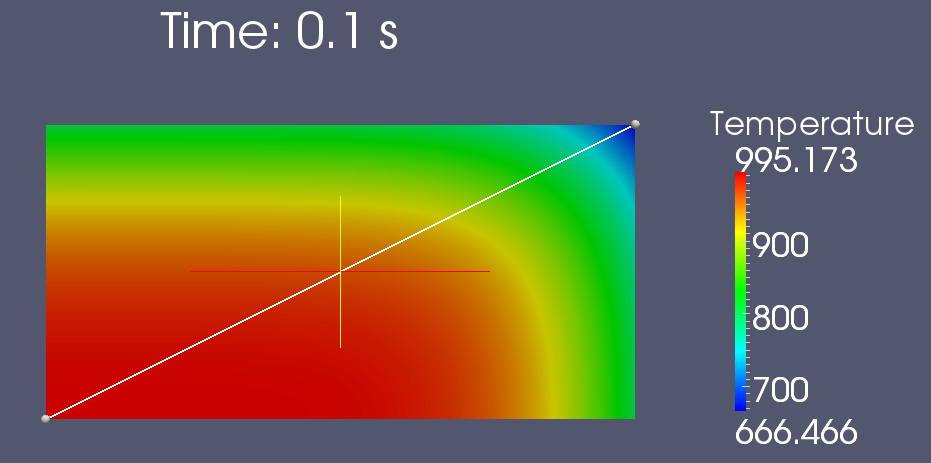
\includegraphics[width=135mm]{./Output/rsz_billet_paraview.png}
\caption{2D: Paraview Output}
\end{figure}

\begin{figure}[ht!]
\centering
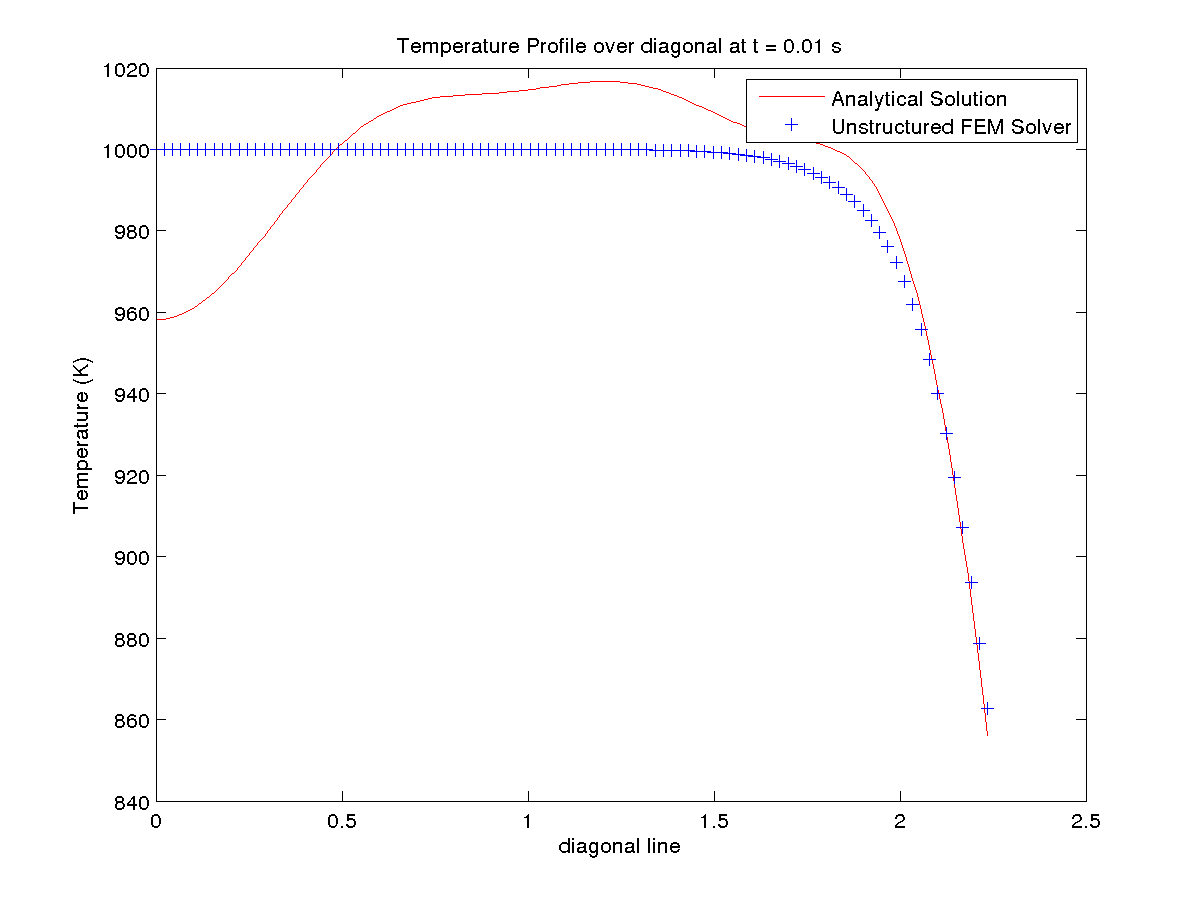
\includegraphics[width=140mm]{./Output/billet001.png}
\caption{2D: Comparison with Analytical solution at time = 0.01 s}
\end{figure}
\begin{figure}[ht!]
\centering
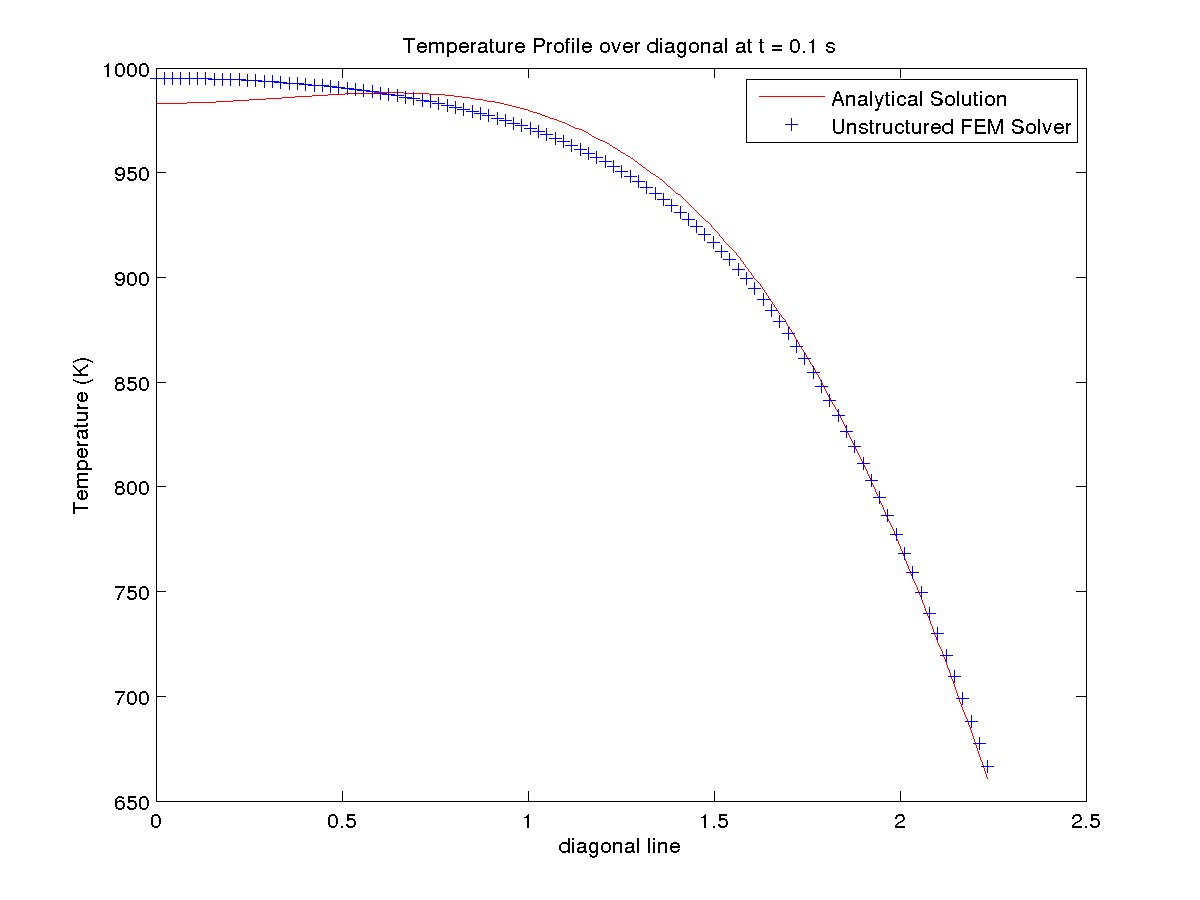
\includegraphics[width=140mm]{./Output/billet01.png}
\caption{2D: Comparison with Analytical solution at time = 0.1 s}
\end{figure}
\begin{figure}[ht!]
\centering
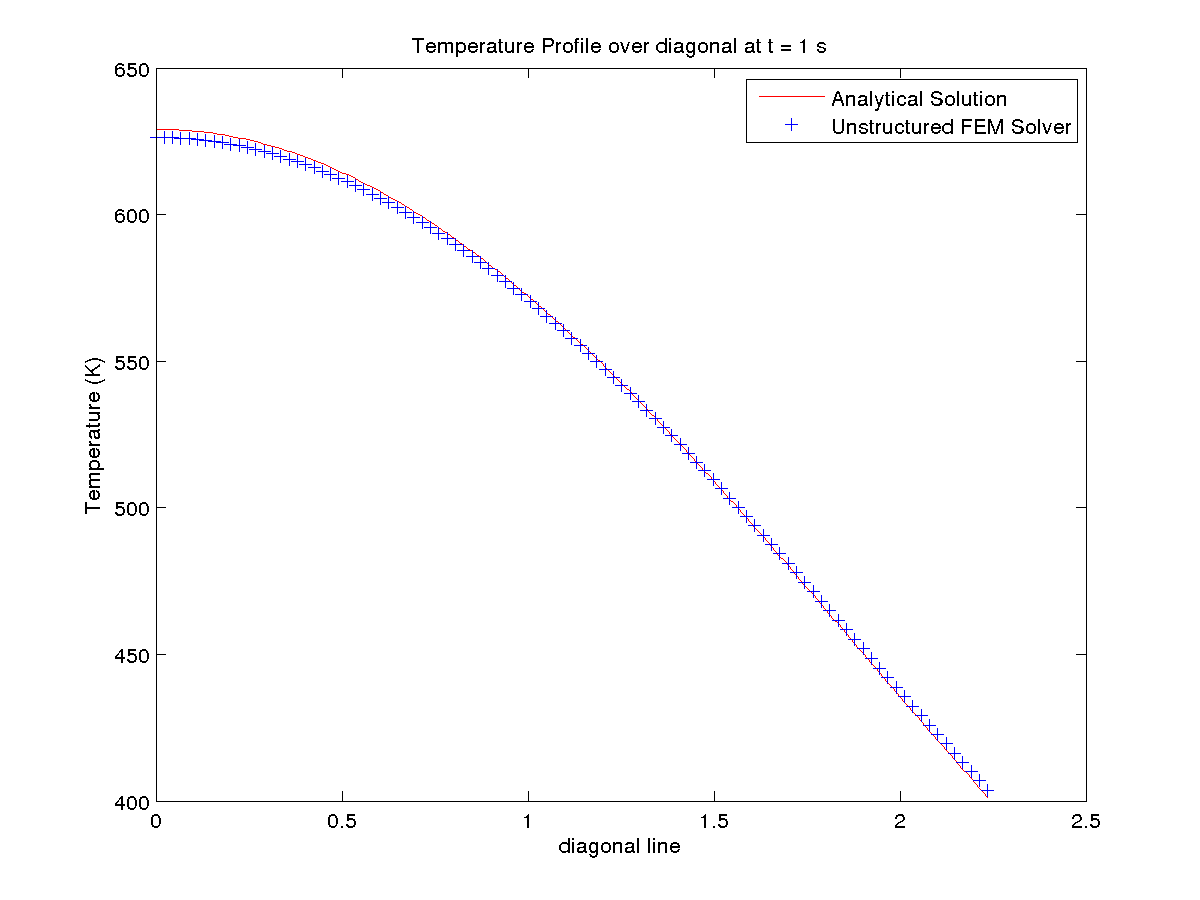
\includegraphics[width=140mm]{./Output/billet1.png}
\caption{2D: Comparison with Analytical solution at time = 1s}
\end{figure}
The plots in figures 11, 12, 13 are plotted along the white line shown in figure 10. In figure 11, the analytical solution exhibits a wavy nature. This is because the solution is in the form of Fourier series with infinite terms, but we have included finite terms for the calculation. This wavy nature is damped at higher times by the exponential factor so we can see more or less smooth behaviour in figures 12 and 13. There is good agreement between the analytical solution and numerical solution in this case too.


\section{Conclusion}
A two dimensional heat diffusion equation is solved numerically using finite element method on unstructured mesh. The FEM uses triangular linear elements. A serial object oriented C++ code is developed based on the FE formulation described in earlier sections. The code is verified and validated against analytical solutions found in \cite{jw}. In the following part, the code will be parallelized.


\bibliographystyle{unsrt}
\bibliography{literature}

\end{document}
